  \documentclass[final]{beamer} 
  % beamer 3.10: do NOT use option hyperref={pdfpagelabels=false} !
  %\documentclass[final,hyperref={pdfpagelabels=false}]{beamer} % beamer 3.07: get rid of beamer warnings
  \mode<presentation> 
  {  %% check http://www-i6.informatik.rwth-aachen.de/~dreuw/latexbeamerposter.php for examples
    \usetheme{Berlin} 
 
 
%\usetheme{I6pd2}
%\definecolor{ljkblue}{rgb}{0.27843, 0.46274, 0.64705} 		
%\definecolor{block_bg}{rgb}{1, 1, 0.8353} 
%\definecolor{ox}{RGB}{207 ,223, 230} 
      
    %% you should define your own theme e.g. for big headlines using your own logos 
  }
  
  \usepackage[english]{babel}
  \usepackage[latin1]{inputenc}
  \usepackage{amsmath,amsthm, amssymb, latexsym}
  %\usepackage{times}\usefonttheme{professionalfonts}  % times is obsolete
  \usefonttheme[onlymath]{serif}
  \boldmath
  \usepackage[orientation=portrait,size=a0,scale=1.4,debug]{beamerposter}                       % e.g. for DIN-A0 poster
  %\usepackage[orientation=portrait,size=a1,scale=1.4,grid,debug]{beamerposter}                  % e.g. for DIN-A1 poster, with optional grid and debug output
  %\usepackage[size=custom,width=200,height=120,scale=2,debug]{beamerposter}                     % e.g. for custom size poster
  %\usepackage[orientation=portrait,size=a0,scale=1.0,printer=rwth-glossy-uv.df]{beamerposter}   % e.g. for DIN-A0 poster with rwth-glossy-uv printer check
  % ...
  %


\setbeamertemplate{bibliography item}[text] 
\bibliographystyle{plain}

%%--------------------------------------------------------------
\def\a{{\alpha }}
\def\b{{\beta }}
\def\d{{\delta }}
\def\e{{\varepsilon}}
\def\o{{\omega}}
\def\ds{\displaystyle}

\def\ha{{\hat{a}}}
\def\hb{{\hat{b}}}
\def\hx{{\hat{x}}}
\def\vf{{\varphi}}
\def\Cau{{{\cal C}^{0,\alpha}(\Gamma_1)}}
\def\Cad{{{\cal C}^{0,\alpha}(\Gamma_2)}}
\def\R{\mathbf R}

%%--------------------------------------------------------------

\definecolor{oxygenorange}{HTML}{F7800A}
\definecolor{oxygengray}{HTML}{686868}
\definecolor{oxygenlightgray}{HTML}{EEEEEE}
\definecolor{oxygenblue}{HTML}{236EAF}
\definecolor{ox}{HTML}{111EAF}
\definecolor{my_purple}{HTML}{ca1885}
%%\definecolor{my_anis}{HTML}{b3ec51}
%%\definecolor{my_anis}{HTML}{c2ed3d}
\definecolor{my_anis}{HTML}{e3ed3d}
\definecolor{my_tilleul}{HTML}{9a9c16}
\definecolor{darkred}{HTML}{c21125}
\definecolor{my_green}{HTML}{88ac0c}

\setbeamercolor*{Title bar}{fg=white}
%%--------------------------------------------------------------
 

%%  \title[Pointwise estimates on the gradients for close-to touching inhomogeneities]{Making
%%Really Fancy Posters with \LaTeX}
%%\author[Oscar Peterson]{}
%%  \institute[Jazz Institute, New York University]{}
%%  \date{Jul. 31th, 2020}
  
  
  
%%--------------------------------------------------------------

  \begin{document}

  \begin{frame}{} 
  
\begin{figure}
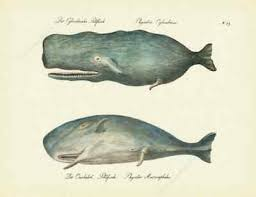
\includegraphics[height=17.0cm]{whale_3.jpeg}
\end{figure}

%%    \vfill
    
%%--------------------------------------------------------------
\begin{block}
{\huge
From Moby Dick (or the Whale)
\medskip}

{\large
Hermann Melville
\hfill Hermann.Merlville@heaven.com}
\vspace*{5mm}

\end{block}

%%--------------------------------------------------------------
%%--------------------------------------------------------------
\begin{block}
{\large 1. Whatever. }

\begin{columns}

\begin{column}{.49\textwidth}
\bigskip

Of the Right Whale, the best outline pictures are in Scoresby; but they are drawn on too small a scale to convey a desirable impression. He has but one picture of whaling scenes, and this is a sad deficiency, because it is by such pictures only, when at all well done, that you can derive anything like a truthful idea of the living whale as seen by his living hunters.

\begin{figure}
%%\includegraphics[height=17.0cm]{../Affiches/AIP_affiche/logo_aip.png}
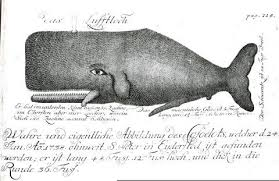
\includegraphics[height=17.0cm]{whale_4.jpeg}
\end{figure}

\end{column}

%%--------------------------------------------------------------
\begin{column}{.49\textwidth}

But, taken for all in all, by far the finest, though in some details not the most correct, presentations of whales and whaling scenes to be anywhere found, are two large French engravings, well executed, and taken from paintings by one Garnery. Respectively, they represent attacks on the Sperm and Right Whale. In the first engraving a noble Sperm Whale is depicted in full majesty of might, just risen beneath the boat from the profundities of the ocean, and bearing high in the air upon his back the terrific wreck of the stoven planks. 

\end{column}

\end{columns}
\end{block}
%%--------------------------------------------------------------
%%--------------------------------------------------------------
\begin{columns}

\begin{column}{.49\textwidth}
\begin{block}{\textcolor{red}{and the next chapter...}}

In the second engraving, the boat is in the act of drawing alongside the barnacled flank of a large running Right Whale, that rolls his black weedy bulk in the sea like some mossy rock-slide from the Patagonian cliffs. His jets are erect, full, and black like soot; so that from so abounding a smoke in the chimney, you would think there must be a brave supper cooking in the great bowels below. Sea fowls are pecking at the small crabs, shell-fish, and other sea candies and maccaroni, which the Right Whale sometimes carries on his pestilent back. And all the while the thick-lipped leviathan is rushing through the deep, leaving tons of tumultuous white curds in his wake, and causing the slight boat to rock in the swells like a skiff caught nigh the paddle-wheels of an ocean steamer. Thus, the foreground is all raging commotion; but behind, in admirable artistic contrast, is the glassy level of a sea becalmed, the drooping unstarched sails of the powerless ship, and the inert mass of a dead whale, a conquered fortress, with the flag of capture lazily hanging from the whale-pole inserted into his spout-hole.

\end{block}
Who Garnery the painter is, or was, I know not. But my life for it he was either practically conversant with his subject, or else marvellously tutored by some experienced whaleman. The French are the lads for painting action. 
\end{column}


%%--------------------------------------------------------------
\begin{column}{.49\textwidth}
\begin{block}{\textcolor{red}{...continues as follows}}
Go and gaze upon all the paintings of Europe, and where will you find such a gallery of living and breathing commotion on canvas, as in that triumphal hall at Versailles; where the beholder fights his way, pell-mell, through the consecutive great battles of France; where every sword seems a flash of the Northern Lights, and the successive armed kings and Emperors dash by, like a charge of crowned centaurs? Not wholly unworthy of a place in that gallery, are these sea battle-pieces of Garnery.


\end{block}
\end{column}

\end{columns}
%%--------------------------------------------------------------
%%--------------------------------------------------------------
\begin{columns}

\begin{column}{.49\textwidth}
\begin{block}



\end{block}
\end{column}


%%--------------------------------------------------------------
\begin{column}{.49\textwidth}
\begin{block}


\end{block}
\end{column}

\end{columns}
%%--------------------------------------------------------------
%%--------------------------------------------------------------
\begin{columns}

\begin{column}{.49\textwidth}
\begin{block}




\end{block}
\end{column}


%%--------------------------------------------------------------
\begin{column}{.49\textwidth}
\begin{block}

\end{block}
\end{column}

\end{columns}
%%--------------------------------------------------------------
%%--------------------------------------------------------------
\begin{columns}

\begin{column}{.49\textwidth}
\begin{block}



\end{block}
\end{column}


%%--------------------------------------------------------------
\begin{column}{.49\textwidth}
\begin{block}
{\large References:}
{\tiny
\begin{thebibliography}{99}

\bibitem{Matthiessen}
Matthiessen, F.O., 
{\em American Renaissance: Art and Expression in the Age of Emerson and Whitman}. 
Oxford University Press (1941).
\\

\bibitem{Melville_mb}
Melville, Herman. 
{\em Moby-Dick or the Whale}, 
The Writings of Herman Melville, Six, Edited by Harrison Hayford, Hershel Parker, and G. Thomas Tanselle, Evanston; Chicago: Northwestern University Press and the Newberry Library, 
ISBN 0810103249,  (1988).
\\

\bibitem{Melville_cp}
Melville, Herman. 
Correspondence. The Writings of Herman Melville Volume Fourteen. Edited by Lynn Horth. Evanston and Chicago: Northwestern University Press and The Newberry Library. ISBN 9780810109957 (1993).
\\

\bibitem{Milder_1}
Milder, Robert. 
{\em The Composition of Moby-Dick: A Review and a Prospect}.
ESQ: A Journal of the American Renaissance (1977).
\\

\bibitem{Milder_2}
Milder, Robert.
{\em Herman Melville}.
In Emory Elliott (General Editor), 
Columbia Literary History of the United States. New York: Columbia University Press. ISBN 0-231-05812-8 (1977).


\end{thebibliography}}

\end{block}
\end{column}

\end{columns}

%%--------------------------------------------------------------
%%--------------------------------------------------------------
\end{frame}
\end{document}
%%--------------------------------------------------------------
%%--------------------------------------------------------------



\begin{columns}
	
\begin{column}{.49\textwidth}
			
\begin{block}{\large }
      \centering
      {\tiny tiny}\par
      {\scriptsize scriptsize}\par
      {\footnotesize footnotesize}\par
      {\normalsize normalsize}\par
      {\large large}\par
      {\Large Large}\par
      {\LARGE LARGE}\par
      {\veryHuge veryHuge}\par
      {\VeryHuge VeryHuge}\par
      {\VERYHuge VERYHuge}\par
 \end{block}
    
 \end{column}
 
\begin{column}
{.49\textwidth}
			
\begin{block}{\large Fontsizes}
      \centering
      {\tiny tiny}\par
      {\scriptsize scriptsize}\par
      {\footnotesize footnotesize}\par
      {\normalsize normalsize}\par
      {\large large}\par
      {\Large Large}\par
      {\LARGE LARGE}\par
      {\veryHuge veryHuge}\par
      {\VeryHuge VeryHuge}\par
      {\VERYHuge VERYHuge}\par
 \end{block}
    
 \end{column}

    
	\end{columns}
%%--------------------------------------------------------------

  
%%--------------------------------------------------------------  
    
    \vfill
    
\end{frame}
%%--------------------------------------------------------------
\end{document}
%%--------------------------------------------------------------


